% $Header: /cvsroot/latex-beamer/latex-beamer/solutions/generic-talks/generic-ornate-15min-45min.en.tex,v 1.5 2007/01/28 20:48:23 tantau Exp $

%\documentclass[mathserif]{beamer}
\documentclass[hyperref={pdfpagelabels=false},slidestop,mathserif,red]{beamer}


% This file is a solution template for:

% - Giving a talk on some subject.
% - The talk is between 15min and 45min long.
% - Style is ornate.



% Copyright 2004 by Till Tantau <tantau@users.sourceforge.net>.
%
% In principle, this file can be redistributed and/or modified under
% the terms of the GNU Public License, version 2.
%
% However, this file is supposed to be a template to be modified
% for your own needs. For this reason, if you use this file as a
% template and not specifically distribute it as part of a another
% package/program, I grant the extra permission to freely copy and
% modify this file as you see fit and even to delete this copyright
% notice. 


\mode<presentation>{
  \usetheme{Copenhagen}
  % or ...
  

  

  \setbeamercovered{transparent}
  % or whatever (possibly just delete it)
}
%\usecolortheme{lily}
\usecolortheme{orchid}

\usepackage[italian]{babel}
% or whatever

\usepackage[latin1]{inputenc}
% or whatever

\usepackage{times}
%\usepackage{cite}
\usepackage[T1]{fontenc}
%\usepackage{fourier}
\usepackage{eulervm}
\usepackage{algorithm}
% Or whatever. Note that the encoding and the font should match. If T1
% does not look nice, try deleting the line with the fontenc.
\usepackage{pgf}

\title[Elaborato di Apprendimento Automatico] % (optional, use only with long paper titles)
{}

\subtitle
{Accelerometer Based Gesture Recognition using HMMs} % (optional)

\author[Andrea~Tarocchi, Marco~Magnatti] % (optional, use only with lots of authors)
{Andrea~Tarocchi, Marco~Magnatti}
% - Use the \inst{?} command only if the authors have different
%   affiliation.


\date[Exam] % (optional)
{8 gennaio 2009}

\subject{Talks}
% This is only inserted into the PDF information catalog. Can be left
% out. 



% If you have a file called "university-logo-filename.xxx", where xxx
% is a graphic format that can be processed by latex or pdflatex,
% resp., then you can add a logo as follows:

 \pgfdeclareimage[height=0.7cm]{university-logo}{university-logo-filename}
 \logo{\pgfuseimage{university-logo}}



% Delete this, if you do not want the table of contents to pop up at
% the beginning of each subsection:


% If you wish to uncover everything in a step-wise fashion, uncomment
% the following command: 

%\beamerdefaultoverlayspecification{<+->}


\begin{document}

\begin{frame}
  \titlepage
\end{frame}

\begin{frame}{Outline}
  \tableofcontents
  % You might wish to add the option [pausesections]
\end{frame}


% Since this a solution template for a generic talk, very little can
% be said about how it should be structured. However, the talk length
% of between 15min and 45min and the theme suggest that you stick to
% the following rules:  

% - Exactly two or three sections (other than the summary).
% - At *most* three subsections per section.
% - Talk about 30s to 2min per frame. So there should be between about
%   15 and 30 frames, all told.

\section{Introduzione}

\begin{frame}{Descrizione del problema}{}
  % - A title should summarize the slide in an understandable fashion
  %   for anyone how does not follow everything on the slide itself.

\begin{block}{}
Da un device dotato di accelerometri si ricevono i dati relativi alle accelerazioni a cui \`e sottoposto durante il moto (lungo le tre coordinate spaziali).
\end{block}
\begin{block}{}
Tale device pu\`o essere impugnato per eseguire gesture.
\end{block}
\begin{block}{}
Il nostro obietivo \`e realizzare un sistema che, dopo adeguato addestramento, sia in grado di riconoscere gesti effettuati tramite tale dispositivo.
\end{block}

\end{frame}


\begin{frame}{Strumenti utilizzati}

\begin{columns}[c]

\begin{column}[T]{2cm}

 \begin{figure}[htbp]
 	\centering
	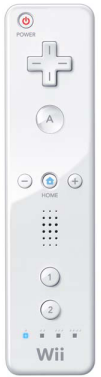
\includegraphics[scale=0.42]{wii.png}
	\label{fig:wii}
 \end{figure}

\end{column}

\begin{column}[t]{9cm}

  \begin{block}{}
	\begin{itemize}
 		\item Device di acquisizione dati: Nintendo Wiimote
		\item Linguaggio di programmazione utilizzato: C/C++
		\item wiiuse: libreria C per comunicazione PC - Wiimote
		\item boost C++: librerie C++ con numerose strutture dati
		\item HMM (Hidden Markov Model): per il riconoscimento
	\end{itemize}
  \end{block}

\end{column}
 
\end{columns}

\end{frame}

\begin{frame}{Struttura generale}

\begin{figure}[htbp]
	\centering
		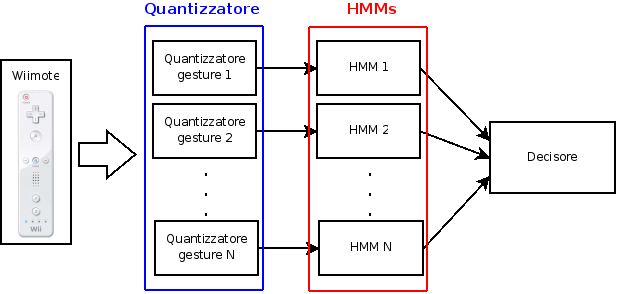
\includegraphics[scale=0.496]{schema.png}
	\label{fig:schema}
\end{figure}

\end{frame}

\section{Quantizzazione dei dati}

\begin{frame}{Quantizzazione con k-means}
\begin{block}{}
Poich\'e i dati in arrivo dal Wiimote sono valori in campo reale compresi tra -4G e +4G, \`e necessaria una discretizzazione prima di poterli sottoporre ad un HMM che, per scelta implementativa, lavora in campo discreto.
\end{block}

\begin{block}{}
La discretizzazione viene fatta tramite l'algoritmo k-means.
\end{block}

\begin{block}{}
Per via sperimentale, si \`e stabilito la posizione iniziale e il numero dei centroidi da utilizzare (e di conseguenza il numero di differenti simboli che l'HMM pu\`o emettere).
\end{block}

\end{frame}

\begin{frame}{Posizione dei centroidi}

\begin{columns}[c]

\begin{column}[T]{7cm}

 \begin{figure}[htbp]
	\centering
	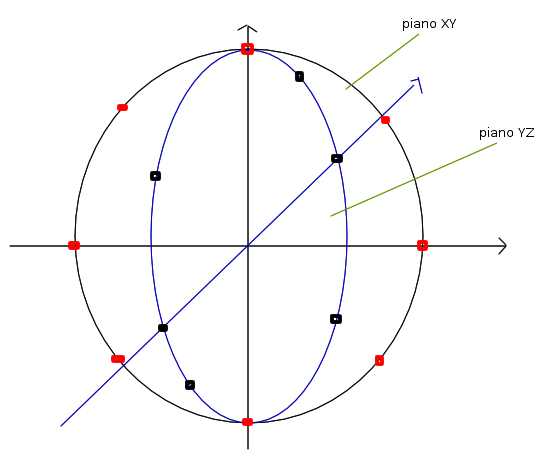
\includegraphics[scale=0.35]{centroidi.png}
	\label{fig:centroidi}
 \end{figure}

\end{column}

\begin{column}[t]{5cm}

 \begin{block}{}
	Possibili approcci alternativi:
	\begin{itemize}
		\item Inizializzazione random
		\item Inizializzazione lungo la direzione del vettore medio
	\end{itemize}

 \end{block}

\end{column}
 
\end{columns}

\end{frame}


\section{HMM}

\subsection{Definizione}

\begin{frame}{HMM}
 \begin{block}{}
  Con HMM \`e possibile affrontare problemi del tipo ``modellare la probabilit\`a $P(X)$ di una sequenza di osservazioni $X$''.\\
Nel nostro caso, le sequenze osservate sono costituite dai vettori di accelerazioni quantizzati in un numero finito di simboli.
 \end{block}

 \begin{block}{}
  Si assume che la sequenza osservata sia generata da una sequenza $S$ di variabili nascoste, chiamate stati.

  Altra assunzione fondamentale \`e che ``il futuro \`e indipendente dal passato, dato il presente'', ovvero vale: \\
$S[t+1] \perp S[1], S[2], \ldots, S[t-1], X[1], X[2], \ldots, X[t] | S[t]$ \\
$X[t+1] \perp S[1], S[2], \ldots, S[t], X[1], X[2], \ldots, X[t] | S[t+1]$
 \end{block}
\end{frame}


\begin{frame}{Elementi di un HMM}
 \begin{block}{}
  Un HMM $\lambda = (\pi, A, B)$ \`e caratterizzato da:
	\begin{itemize}
		\item $N$, il numero di stati (nascosti) nel modello
		\item $M$, il numero di distinti simboli osservabili (alfabeto)
	 \item $\pi = \{\pi_{i}\}$, con $\pi_{i} = P[q_{1} = S_{i}]$, il vettore delle probabilit\`a iniziali degli stati
 	 \item $A = \{a_{ij}\}$, con $a_{ij} = P[q_{t+1} = S_{j} | q_{t} = S_{i}]$, la matrice di transizione tra gli stati
 	 \item $B = \{b_{jk}\}$, con $b_{jk} = P[osservo\ il\ simbolo\ v_{k}\ al\ tempo\ t | q_{t} = S_{j}]$, la matrice di emissione (essendo il modello stazionario, $B$ \`e indipendente dal tempo)
	\end{itemize}

 \end{block}

\end{frame}

\begin{frame}{I 3 problemi di base}
 \begin{block}{}
  Ci sono 3 problemi la cui risoluzione \`e indispensabile affinch\`e il modello risulti utilizzabile in applicazioni reali:
	\begin{enumerate}
	 \item \textit{\textbf{Prediction}}: data una sequenza di simboli $V = \{v_{1}, \ldots, v_{T}\}$ e un modello $\lambda$, calcolare la \textit{likelihood} $P(V|\lambda)$
	 \item \textbf{\textit{Learning}}: date una o pi\`u sequenze di training, calcolare i parametri del modello $\lambda$ che meglio spiegano i dati
	 \item \textit{\textbf{Decoding}}: data una sequenza di simboli $V = \{v_{1}, \ldots, v_{T}\}$ e un modello $\lambda$, determinare la pi\`u probabile sequenza di stati che possa aver generato i simboli dati
	\end{enumerate}
 \end{block}
\end{frame}

\subsection{Prediction}

\begin{frame}{Soluzione al problema 1}
 \begin{block}{}
  Vogliamo calcolare la probabilit\`a della sequenza di osservazioni $O = (O_{1}, O_{2}, \ldots, O_{T}$) dato il modello $\lambda$, ossia $P(O|\lambda)$.
 \end{block}
\begin{block}{}
Il modo pi\`u immediato di farlo comporterebbe enumerare tutte le possibili sequenze di stati $Q_{k}$, sommando poi le probabilit\`a condizionate $P(O|Q_{k},\lambda) \cdot P(Q_{k}|\lambda)$, ma arriverebbe ad avere una complessit\`a intrattabile (dell'ordine di $2T \cdot N^{T}$).
 \end{block}
\begin{block}{}
Pertanto, si ricorre alla \textit{Forward-Backward Procedure}, che vedremo avere una complessit\`a dell'ordine di $N^2 \cdot T$.
 \end{block}

\end{frame}

\begin{frame}{The Forward-Backward Procedure}
 \begin{block}{}
  Definiamo la variabile forward $\alpha_{t}(i)$ come:
	\begin{center}
	$\alpha_{t}(i) = P(O_{1}, O_{2}, \cdots, O_{t}, q_{t} = S_{i}|\lambda)$
	\end{center}
ossia la probabilit\`a di osservare $O_{1}, \cdots, O_{t}$ (sequenza parziale) ed essere nello stato $S_{i}$ al tempo $t$, dato il modello $\lambda$.
 \end{block}
 \begin{block}{}
	\pgfputat{\pgfxy(8.5,-2.2)}{\pgfbox[left,base]{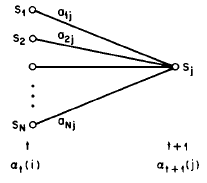
\includegraphics[width=2.2cm]{alpha.png}}}
% \begin{columns}[c]
%   \begin{column}[t]{8.5cm}
	Procediamo per induzione su $\alpha_{t}(i)$:
	\begin{enumerate}
 	\item Inizializzazione: $\alpha_{1}(i) = \pi_{i}b_{i}(O_{1})$
	\item Induzione: $\alpha_{t+1}(j) = (\sum_{i = 1}^{N} \alpha_{t}(i)a_{ij}) \cdot b_{j}(O_{t+1})$
	\item Terminazione: $P(O|\lambda) = \sum_{i=1}^{N}\alpha_{T}(i)$
	\end{enumerate}
%   \end{column}
%  \begin{column}[T]{1.5cm}
%	\begin{figure}[ht]
%	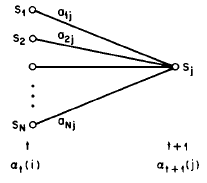
\includegraphics[scale=0.25]{alpha.png}
%	\label{fig:alpha}
% \end{figure}
%   \end{column}
% \end{columns}
 \end{block}

\end{frame}


\begin{frame}
 \begin{block}{}
  Definiamo la variabile backward $\beta_{t}(i)$ come segue:
\begin{center}
 $\beta_{t}(i) = P(O_{t+1}, O_{t+2}, \ldots, O_{T} | q_{t} = S_{i}, \lambda)$
\end{center}
ossia, la probabilit\`a di osservare la parte finale della sequenza, da $t+1$ fino alla fine, dato lo stato $S_{i}$ al tempo $t$ e il modello $\lambda$.
 \end{block}
\begin{block}{}
	\pgfputat{\pgfxy(8.5,-1.7)}{\pgfbox[left,base]{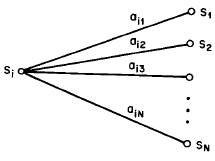
\includegraphics[width=2.2cm]{beta.png}}}
% \begin{columns}[c]
%   \begin{column}[h]{8cm}
	Procediamo per induzione su $\beta_{t}(i)$:
	\begin{enumerate}
 	\item Inizializzazione: $\beta_{T}(i) = 1$
	\item Induzione: $\beta_{t}(i) = \sum_{j = 1}^{N} a_{ij}b_{j}(O_{t+1})\beta_{t+1}(j)$
	\end{enumerate}
    
%   \end{column}
%   \begin{column}[T]{2cm}
%	\begin{figure}[ht]
%	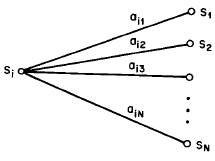
\includegraphics[scale=0.3]{beta.png}
%	\label{fig:beta}
% \end{figure}
%   \end{column}
% \end{columns}
\end{block}
 
\end{frame}



\subsection{Learning}

\begin{frame}[shrink]{Soluzione al problema 2}
 \begin{block}{}
  Non si conosce un metodo analitico per determinare il modello che massimizza la probabilit\`a della sequenza data.\\
  Si pu\`o usare l'algoritmo di Baum-Welch per massimizzare localmente $P(O|\lambda)$.
 \end{block}
 \begin{block}{}
  Definiamo la variabile $\xi_{t}(i,j) = P(q_{t} = S_{i}, q_{t+1} = S_{j}|O,\lambda)$ \\
ovvero la probabilit\`a di trovarsi nello stato $S_{i}$ al tempo $t$ e nello stato $S_{j}$ al tempo $t+1$, dati $O$ e $\lambda$.\\
Possiamo esprimerla in funzione delle variabili forward e backward:
\begin{center}
$ \xi_{t}(i,j) = \frac{\alpha_{t}(i)a_{ij}b_{j}(O_{t+1})\beta_{t+1}(j)}{P(O|\lambda)} $       \end{center}
\end{block}
\end{frame}

\begin{frame}{}
\begin{block}{}
Definiamo la variabile $\gamma_{t}(i) = P(q_{t} = S_{i}|O,\lambda)$, ossia la probabilit\`a di trovarsi nello stato $S_{i}$ al tempo $t$ dati $O$ e $\lambda$.\\
Questa pu\`o essere ricavata dalle variabili forward e backward come segue:
 \begin{equation}
	\gamma_{t}(i) = \frac{\alpha_{t}(i)\beta_{t}(i)}{P(O|\lambda)}
\end{equation}
e in funzione della variabile $\xi_{t}(i,j)$:
 \begin{equation}
	\gamma_{t}(i) = \sum_{j=1}^{N}\xi_{t}(i,j)
\end{equation}

\end{block}
\end{frame}

\begin{frame}
 \begin{block}{}
  Sommando $\gamma_{t}(i)$ rispetto a $t$, si ottiene una quantit\`a che indica il numero atteso di volte che passeremo per lo stato $S_{i}$. Analogamente, la somma di $\xi_{t}(i,j)$ su $t$ pu\`o essere interpretata come il numero (atteso) di transizioni tra $S_{i}$ e $S_{j}$. Pertanto:
\begin{center}
 $\sum_{t=1}^{T-1}\gamma_{t}(i) =$ numero atteso di transizioni da $S_{i}$
\end{center}
\begin{center}
 $\sum_{t=1}^{T-1}\xi_{t}(i,j) =$ numero atteso di transizioni da $S_{i}$ a $S_{j}$
\end{center}
 \end{block}

\begin{block}{}
 Usando le formule appena introdotte e il concetto di conteggiare le occorrenze degli eventi ai fini di stimare le probabilit\`a, \`e possibile fornire un metodo per la ristima dei parametri dell'HMM.
\end{block}
\end{frame}

\begin{frame}
 \begin{block}{Formule di ristima dei parametri}
 \begin{center}
$\overline{\pi_{i}} = numero\ atteso\ di\ volte\ in\ stato\ S_{i}\ al\ tempo\ 1 = \gamma_{1}(i)$
\end{center}

\begin{center}
 $\overline{a_{ij}} = \dfrac{numero\ atteso\ di\ transizioni\ da\ S_{i}\ a\ S_{j}}{numero\ atteso\ di\ transizioni\ da\ S_{i}} = \frac{\sum_{t=1}^{T-1}\xi_{t}(i,j)}{\sum_{t=1}^{T-1}\gamma_{t}(i)}$
\end{center}

\begin{center}
 $ \overline{b_{j}(k)} = \dfrac{numero\ atteso\ di\ volte\ in\ S_{j}\ osservando\ il\ simbolo\ v_{k}}{numero\ atteso\ di\ volte\ nello\ stato\ S_{j}} = \frac{\sum_{t=1, s.t. O_{t} = v_{k}}^{T}\gamma_{t}(j)}{\sum_{t=1}^{T}\gamma_{t}(j)}$
\end{center}

 \end{block}
\end{frame}


\subsection{Decoding}

\begin{frame}{Soluzione al problema 3}
\begin{block}{}
Ci sono differenti modi per trovare la sequenza di stati \textit{``ottimale''} data la sequenza di osservazioni.
\end{block}

\begin{block}{}
Un possibile criterio \`e di scegliere gli stati $q_{t}$ che sono individualmente pi\`u probabili 
\end{block}

\begin{block}{}
Utilizzando le variabili $\gamma_{t}(i)$ prima definite si pu\`o trovare lo stato $q_{t}$ pi\`u probabile al tempo $t$ come:
\begin{center}
	$q_{t}=\underset{1 \leq i \leq N}{\arg\max}[\gamma_{t}(i)],\ \ \ 1\leq t \leq T$
\end{center}
\end{block}

\end{frame}


\begin{frame}
\begin{block}{}
Un criterio largamente usato \`e quello di trovare la singola miglior sequenza ossia massimizzare $P(Q|O,\lambda)$ che \`e equivalente a massimizzare $P(Q,O|\lambda)$.
\end{block}

\begin{block}{}
Per fare questo si utilizza l'algoritmo di Viterbi.\\
E' utile introdurre la quantit\`a: 
\begin{center}
$\delta_{t}(i) = \underset{q_{1},q_{2},\ldots,q_{t-1}}{\max}P(q_{1},q_{2},\ldots,q_{t}=i,O_{1}O_{2}\cdots O_{t}|\lambda)$
\end{center}
Ossia \`e la pi\`u alta probabilit\`a lungo un singolo cammino al tempo $t$ che tiene conto delle prime $t$ osservazioni e finisce nello stato $S_{i}$
\end{block}

\end{frame}

\begin{frame}
\begin{block}{Algoritmo di Viterbi}
\begin{enumerate}
\item Inizializzazione:
	\begin{itemize}
 	\item $\delta_{1}(i)=\pi_{i}b_{i}(O_{1}),\ \ \psi_{1}(i)=0,\ \ \ \ 1\leq i \leq N$  
	\end{itemize}
\item Ricorsione:
	\begin{itemize}
 	\item $\delta_{t}(j)=\underset{1\leq i \leq N}{\max}[\delta_{t-1}(i)a_{ij}]b_{j}(O_{t}),\ \ \ 1\leq j \leq N$
	\item $\psi_{t}(j)=\underset{1\leq i \leq N}{\arg\max}[\delta_{t-1}a_{ij}],\ \ \ \ \ \ \ \ \ \ \ \ 2\leq t \leq T$
	\end{itemize}
\item Terminazione
	\begin{itemize}
 	\item $P^*=\underset{1\leq i \leq N}{\max}[\delta_{T}(i)]$
	\item $q_{T}^*=\underset{1\leq i \leq N}{\arg\max}[\delta_{T}(i)]$
	\end{itemize}
\item Sequenza degli stati:
	\begin{itemize}
 	\item $q_{t}^*=\psi_{t+1}(q_{t+1}^*),\ \ t = T-1,T-2,\ldots1$
	\end{itemize}
\end{enumerate}
\end{block}
\end{frame}

\section{Decisore}

\begin{frame}{Riconoscimento della gesture}
\begin{block}{}
\begin{itemize}
 \item Per ciascuna classe di gesture che si intende riconoscere, si addestra un distinto HMM.
 \item Data una gesture $O$ da riconoscere, questa viene sottoposta a ciascun modello $\lambda_{i}$, e tramite la procedura Forward si calcolano le probabilit\`a $P(O|\lambda_{i})$.
 \item La gesture viene attribuita alla classe relativa all'HMM che produce la probabilit\`a maggiore.
\end{itemize}

\end{block}
\end{frame}

\begin{frame}
\begin{block}{}
 Quello che vogliamo sapere \`e la probabilit\`a che una data sequenza $O$ appartenga alla classe $C_{i}$, ovvero $P(C_{i}|O)$.
\end{block}
\begin{block}{}
 La procedura Forward ci permette invece di determinare $P(O|C_{i})$, ma vale
\begin{center}$P(C_{i}|O) = \frac{P(O|C_{i})P(C_{i})}{P(O)}$\end{center}
\end{block}
\begin{block}{}
 Pertanto, per prendere la decisione, dovremmo scegliere la $P(O|C_{i})P(C_{i})$ massima. Possiamo per\`o limitarci a decidere sulla base della sola $P(O|C_{i})$ in quanto si assume che ciascuna classe di gesture sia equiprobabile.
\end{block}
\end{frame}

\section{Test e risultati}

\begin{frame}{Test eseguiti}
\begin{block}{}
\begin{itemize}
\item Si \`e messo alla prova il software su 3 classi di gesture: triangolo, quadrato e zeta.
\item La topologia utilizzata \`e quella left-to-right, con span 1 e 9 diversi stati (combinazione di parametri che ha prodotto i risultati migliori).
\item Il dataset utilizzato comprende circa 50 gesture per classe, eseguite da 2 persone distinte.
\item La valutazione delle prestazioni \`e stata effettuata tramite 3-fold cross validation.
\end{itemize}

\end{block}
\end{frame}

\begin{frame}[shrink]{Risultati}
\begin{block}{}
\begin{columns}[T]
\begin{column}[C]{2cm}
\ \\
\alert{Triangolo:}\\
51 su 51 100\%
\end{column}
\begin{column}[TL]{8cm}
\begin{itemize}
 \item fold 1: 17 su 17
 \item fold 2: 17 su 17
 \item fold 3: 17 su 17
\end{itemize}
\end{column}
\end{columns}
\pgfputat{\pgfxy(8.5,-0.05)}{\pgfbox[left,base]{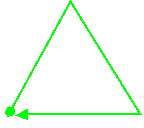
\includegraphics[width=1.6cm]{triangolo.png}}}\end{block}

\begin{block}{}
\begin{columns}[T]
\begin{column}[C]{2cm}
\ \\
\alert{Quadrato:}\\
47 su 51 92\%
\end{column}
\begin{column}[TL]{8cm}
\begin{itemize}
 \item fold 1: 16 su 17
 \item fold 2: 15 su 17
 \item fold 3: 16 su 17
\end{itemize}
\end{column}
\end{columns}
\pgfputat{\pgfxy(8.5,-0.01)}{\pgfbox[left,base]{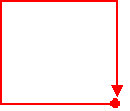
\includegraphics[width=1.6cm]{quadrato.png}}}
\end{block}

\begin{block}{}
\begin{columns}[T]
\begin{column}[C]{2cm}
\ \\
\alert{Zeta:}\\
51 su 51 100\%
\end{column}
\begin{column}[TL]{8cm}
\begin{itemize}
 \item fold 1: 17 su 17
 \item fold 2: 17 su 17
 \item fold 3: 17 su 17
\end{itemize}
\end{column}
\end{columns}
\pgfputat{\pgfxy(8.5,-0.05)}{\pgfbox[left,base]{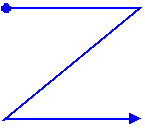
\includegraphics[width=1.6cm]{zeta.png}}}\end{block}
%  \begin{figure}[ht]
%	\centering
%	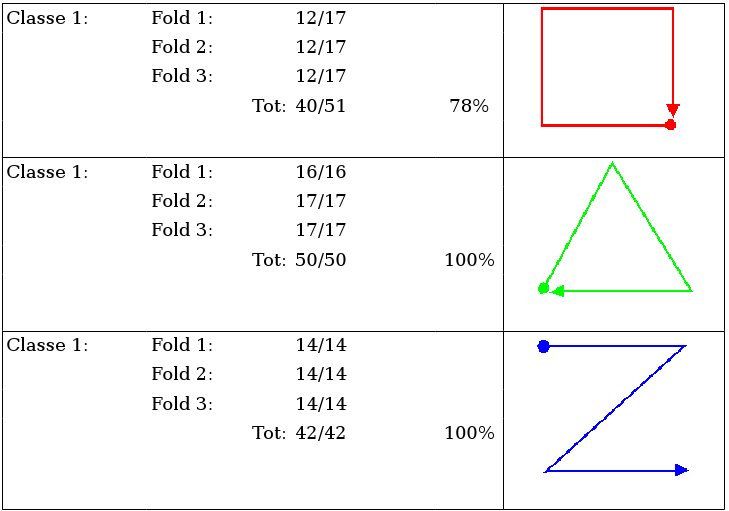
\includegraphics[scale=0.32]{risultati.png}
%	\label{fig:risultati}
%  \end{figure}
\end{frame}

\begin{frame}
\begin{columns}

 \begin{column}[C]{15cm}
 \pgfputat{\pgfxy(0.33,-3.1)}{\pgfbox[left,base]{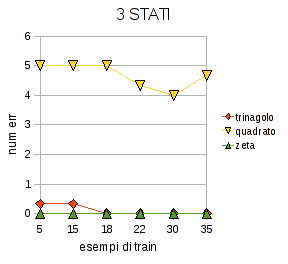
\includegraphics[width=4cm]{risultati-img1.png}}}
 \pgfputat{\pgfxy(4.33,-3.1)}{\pgfbox[left,base]{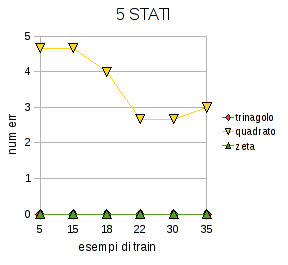
\includegraphics[width=4cm]{risultati-img2.png}}}
 \pgfputat{\pgfxy(8.33,-3.1)}{\pgfbox[left,base]{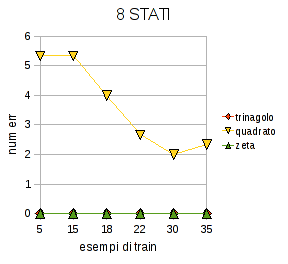
\includegraphics[width=4cm]{risultati-img3.png}}}
\pgfputat{\pgfxy(0,-7)}{\pgfbox[left,base]{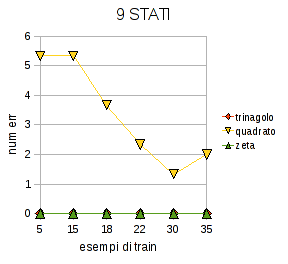
\includegraphics[width=4cm]{risultati-img4.png}}} 
\pgfputat{\pgfxy(4,-7)}{\pgfbox[left,base]{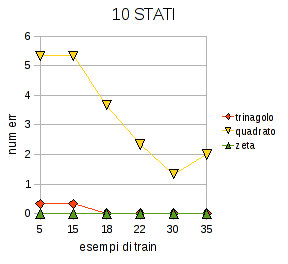
\includegraphics[width=4cm]{risultati-img5.png}}}
\end{column}

\end{columns}
\end{frame}

\begin{frame}
 \begin{block}{}
  Tramite i test effettuati si sono individuati i parametri che garantivano risultati migliori.
 \end{block}
 
 \begin{block}{}
  Utilizzando tali parametri, \`e stato realizzato un applicativo che effettua il riconoscimento delle gesture ``live''.
 \end{block}
 
 \begin{block}{}
  L'accuratezza nel riconoscimento delle 3 gesture tramite tale applicativo \`e risultata paragonabile a quella ottenuta nei test precedenti.
 \end{block}

 
\end{frame}


\begin{frame}
	\frametitle{Bibliografia}
	
		\begin{thebibliography}{}
		%
%			\bibitem<1->[Solomaa, 1973]{Solomaa1973}
%				A.~Salomaa.
%				\newblock {\em Formal Languages}.
%				\newblock Academic Press, 1973.
				\footnotesize
				
				\bibitem<1->[Rabiner, 1989]{Rabiner1973}
			 	Lawrence R. Rabiner
				\newblock {\em A Tutorial on Hidden Markov Models and Selected Applications in Speech Recognition}.
				
				\bibitem<1->[HAH, 2001]{HAH2001}
				Xuedong Huang, Alex Acero, Hsiao-Wuen Hon
				\newblock {\em Spoken Language processing. A guide to theory, algorithm and system development.}
				\newblock Prentice Hall, 2001
				
				\bibitem<1->[Mantyla, 2001]{Mantyla2001}
				Vesa-Matti M\"{a}ntyl\"{a} 
				\newblock {\em Discrete Hidden Markov Models with application to isolated user-dependent hand gesture recognition}.
				\newblock VTT Publications, 2001


\end{thebibliography}
\end{frame}

\end{document}

